\documentclass[tikz]{standalone}
\usepackage{tikz}
\usepackage{mathtools}
\usetikzlibrary{shapes.geometric, arrows, backgrounds, positioning, matrix,shapes,chains,calc, trees, shapes, shapes.multipart, shadows, matrix, decorations.pathreplacing, decorations.pathmorphing}
\tikzstyle{startstop} = [rectangle, rounded corners, minimum width=3cm, minimum height=1cm,text centered, draw=black, fill=red!30]
\tikzstyle{io} = [ellipse, minimum width=3cm, minimum height=1cm, text centered, draw=black, fill=orange!30]
\tikzstyle{process} = [rectangle, minimum width=3cm, minimum height=1cm, text centered, draw=black, fill=blue!30]
\tikzstyle{decision} = [diamond, minimum width=3cm, minimum height=1cm, text centered, draw=black, fill=green!30]
\tikzstyle{arrow} = [thick,->,>=stealth]
\tikzset{
    descr/.style={
        fill=white,
        inner sep=2.5pt
    },
    connector/.style={
     -latex,
     font=\scriptsize
    },
    rectangle connector/.style={
        connector,
        to path={(\tikztostart) -- ++(#1,0pt) \tikztonodes |- (\tikztotarget) },
        pos=0.5
    },
    rectangle connector/.default=-2cm,
    straight connector/.style={
        connector,
        to path=--(\tikztotarget) \tikztonodes
    }
    }
    \tikzstyle{line} = [draw, -latex']
\begin{document}
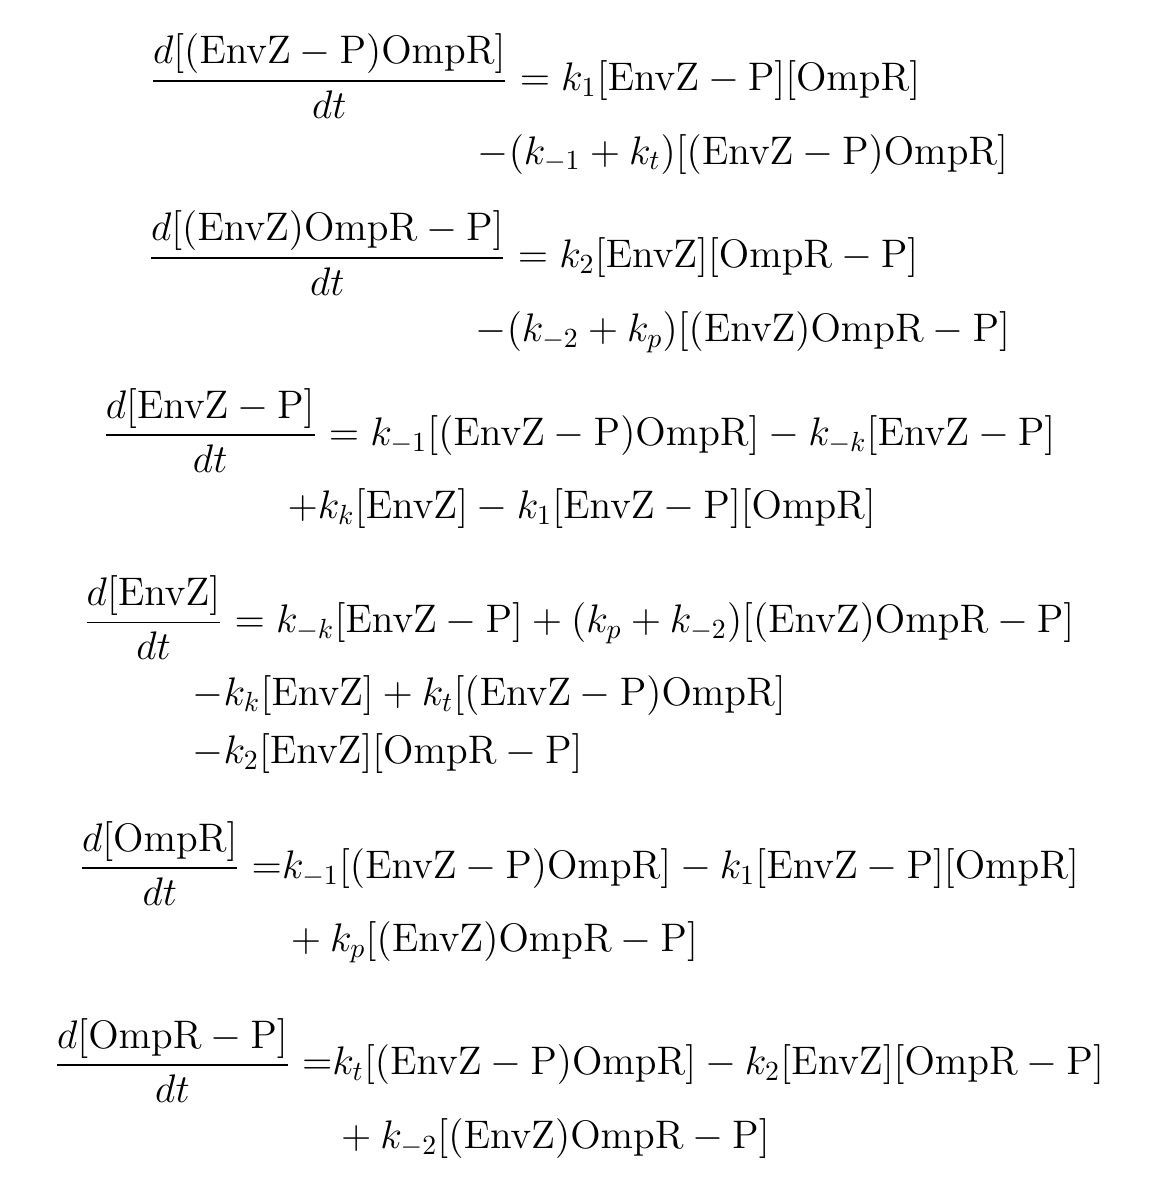
\begin{tikzpicture}[scale = 1]
\Large
\useasboundingbox (-7, -5) rectangle (7, 9.5);

  \coordinate (first) at (0, 8.5);
  \node at (first) {
   $\begin{aligned}
     \frac{d[\mathrm{(EnvZ-P)OmpR}]}{dt} &=  k_1[\mathrm{EnvZ-P}][\mathrm{OmpR}] \\ -& (k_{-1}+k_t)[\mathrm{(EnvZ-P)OmpR}]
    \end{aligned}$ 
  };
  
  \node at ($(first) + (0, -2.25)$) {
   $\begin{aligned}
     \frac{d[\mathrm{(EnvZ)OmpR-P}]}{dt} &=  k_2[\mathrm{EnvZ}][\mathrm{OmpR-P}] \\ - & (k_{-2}+k_p)[\mathrm{(EnvZ)OmpR-P}]
    \end{aligned}$ 
  };
  
  \node at ($(first) + (0, -4.5)$) {
   $\begin{aligned}
     \frac{d[\mathrm{EnvZ-P}]}{dt} &=  k_{-1}[\mathrm{(EnvZ-P)OmpR}]-k_{-k}[\mathrm{EnvZ-P}]  \\
     +& k_k[\mathrm{EnvZ}] - k_{1}[\mathrm{EnvZ-P}][\mathrm{OmpR}]
    \end{aligned}$ 
  };
  
  \node at ($(first) + (0, -7.25)$) {
   $\begin{aligned}
     \frac{d[\mathrm{EnvZ}]}{dt} &=  k_{-k}[\mathrm{EnvZ-P}] + (k_p+k_{-2})[\mathrm{(EnvZ)OmpR-P}] \\
     -&k_{k}[\mathrm{EnvZ}] +k_t[\mathrm{(EnvZ-P)OmpR}] \\
     -& k_{2}[\mathrm{EnvZ}][\mathrm{OmpR-P}]
    \end{aligned}$ 
  };
  
  \node at ($(first) + (0, -10)$) {
   $\begin{aligned}
     \frac{d[\mathrm{OmpR}]}{dt} =&  k_{-1}[\mathrm{(EnvZ-P)OmpR}]-k_{1}[\mathrm{EnvZ-P}][\mathrm{OmpR}]  \\
     &+ k_p[\mathrm{(EnvZ)OmpR-P}] 
    \end{aligned}$ 
  };
  
  \node at ($(first) + (0, -12.5)$) {
   $\begin{aligned}
     \frac{d[\mathrm{OmpR-P}]}{dt} =&  k_{t}[\mathrm{(EnvZ-P)OmpR}]-k_{2}[\mathrm{EnvZ}][\mathrm{OmpR-P}] \\
     &+ k_{-2}[\mathrm{(EnvZ)OmpR-P}] 
    \end{aligned}$ 
  };
%   \node[single arrow, right = 4.25cm of data, draw, right color = red!35!white, left color = red!10!white, minimum width = 3cm, rounded corners, shading angle=90+45] {\Large Time-Course \\ \vspace{1mm} \Large Data};
 
  
%   \coordinate (aim) at ($(im) - (12,0)$);
%   \node[single arrow, above = .75cm of aim, draw, right color = red!20!white, left color = red!05!white, shading angle=90+45, minimum height = 3cm, minimum width = 3.75cm, shape border rotate=270, align = center, rounded corners] {$\qquad$};


\end{tikzpicture}
\end{document}